\documentclass[12pt]{article}
\usepackage[margin=1in]{geometry}
\usepackage{graphicx}
\usepackage{booktabs}
\usepackage{amsmath}
\usepackage{amssymb}
\usepackage{float}
\usepackage{caption}
\usepackage{setspace}
\usepackage[most]{tcolorbox}
\captionsetup{font=small, labelfont=bf, skip=6pt}
\onehalfspacing

\newtcolorbox{explain}{%
  colback=black!3,
  colframe=black!25,
  boxrule=0.5pt,
  arc=1pt,
  left=8pt,
  right=8pt,
  top=5pt,
  bottom=5pt,
  before skip=6pt,
  after skip=12pt,
  fontupper=\normalsize
}

\title{Classical Baselines\\[0.2em]
\large Bitcoin realized volatility}
\author{Volatility forecasting project}
\date{29 September 2026}

\begin{document}
\maketitle

\noindent
Results for Naive, HAR, ARIMA, and GARCH under the frozen Protocol~B
(\texttt{eval\_freeze/}). LSTM results are in \texttt{lstm\_report.pdf}.
Script: \texttt{models/run\_baselines.py}.

\section{Protocol reminder}
Tune on train (AIC where needed) $\rightarrow$ final fit on train+val $\rightarrow$ score on test
(2024-01-01 through 2026-09-25, $n=999$).
Metrics: RMSE and MAE on $\log\mathrm{RV}$; MAPE and QLIKE on RV.

\section{Naive}
\[
\hat y_t=\log\mathrm{RV}_t.
\]
\begin{explain}
No parameters. Test RMSE $0.560$, MAE $0.444$, QLIKE $0.161$. Floor for the ladder.
\end{explain}

\section{HAR}
\[
\hat y_t
=
\hat c
+ \hat\beta_d\log\mathrm{RV}^{(d)}_t
+ \hat\beta_w\log\mathrm{RV}^{(w)}_t
+ \hat\beta_m\log\mathrm{RV}^{(m)}_t.
\]
OLS on train+val ($n=2269$):
$\hat c=-0.341$, $\hat\beta_d=0.299$, $\hat\beta_w=0.457$, $\hat\beta_m=0.151$.
\begin{explain}
Weekly component carries the largest weight. Test RMSE $0.458$, MAE $0.354$, QLIKE $0.101$ --- best classical score.
\end{explain}

\section{ARIMA}
Order selected by AIC on train: ARIMA$(3,0,3)$. Refit on train+val; one-step forecasts on test with frozen parameters (state updated by appending realized $\log\mathrm{RV}$).
\begin{explain}
Beats Naive (RMSE $0.518$, MAE $0.407$, QLIKE $0.132$) but trails HAR. Structured day/week/month lags beat a generic ARMA on this target.
\end{explain}

\section{GARCH}
AIC on train over $\{(1,1),(1,2),(2,1)\}$ selected GARCH$(2,1)$ on daily returns (percent scale).
Parameters refit on train+val; one-step $\hat\sigma_{t+1}$ walked forward on the return path with frozen coefficients.
Scored against realized $\mathrm{RV}_{t+1}$ / $\log\mathrm{RV}_{t+1}$.
\begin{explain}
Test RMSE $0.656$, MAE $0.523$, QLIKE $0.161$.
GARCH forecasts conditional return volatility. Scored against intraday realized volatility, it trails the lagged-RV models on RMSE and MAE.
\end{explain}

\section{Test leaderboard}
\begin{table}[H]
\centering
\begin{tabular}{lcccc}
\toprule
Model & RMSE (log) & MAE (log) & MAPE (\%) & QLIKE \\
\midrule
Naive & 0.560 & 0.444 & 51.1 & 0.161 \\
HAR & \textbf{0.458} & \textbf{0.354} & \textbf{40.7} & \textbf{0.101} \\
ARIMA$(3,0,3)$ & 0.518 & 0.407 & 47.4 & 0.132 \\
GARCH$(2,1)$ & 0.656 & 0.523 & 82.9 & 0.161 \\
\bottomrule
\end{tabular}
\caption{Test metrics. RMSE and MAE on $\log\mathrm{RV}$; MAPE and QLIKE on RV. Bold = best among classical baselines.}
\end{table}
\begin{figure}[H]
\centering
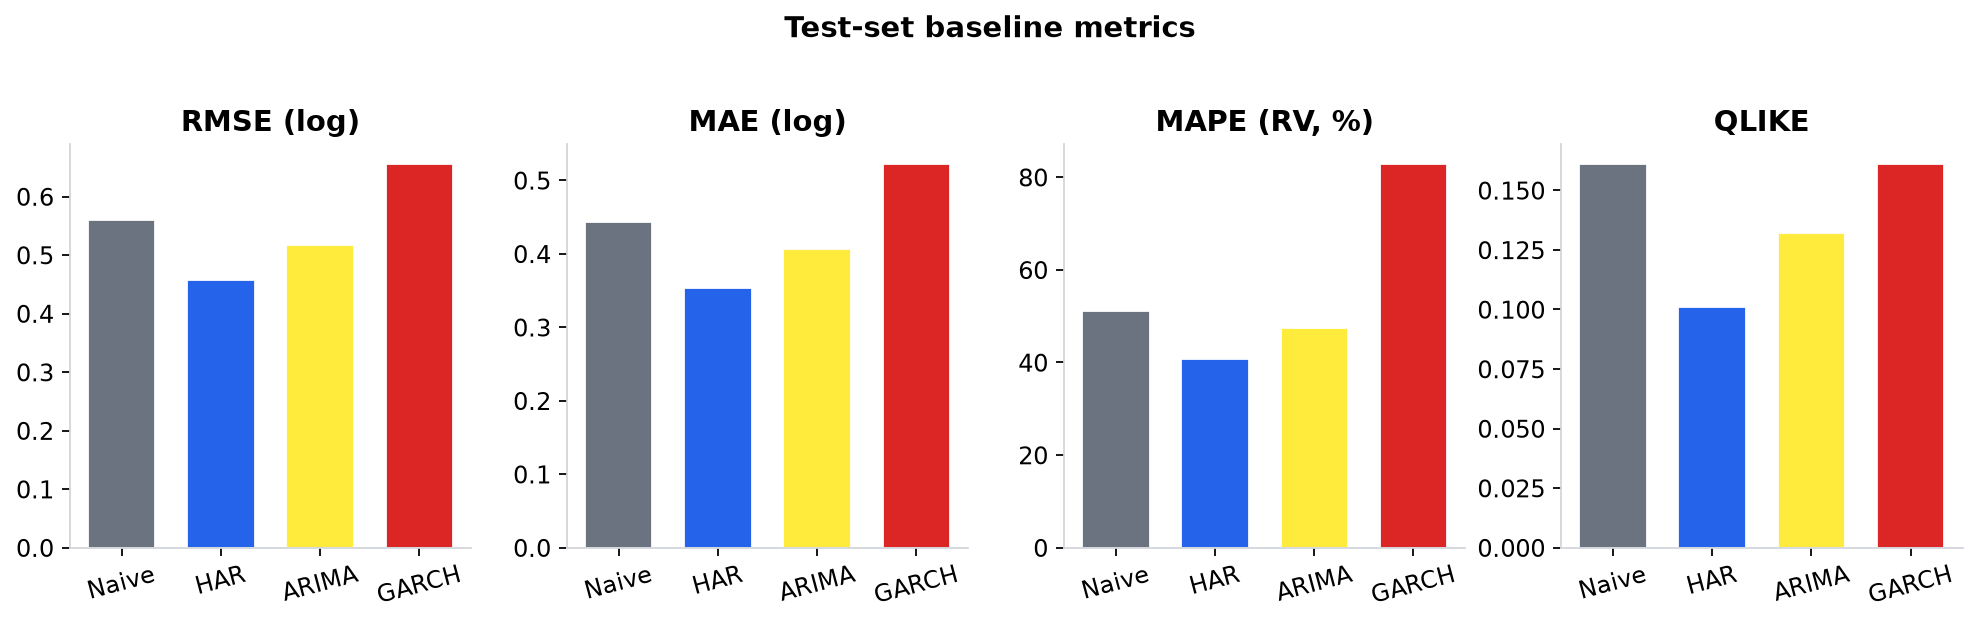
\includegraphics[width=\textwidth]{figures/baseline_metrics.png}
\caption{Test metrics by model.}
\end{figure}
\begin{figure}[H]
\centering
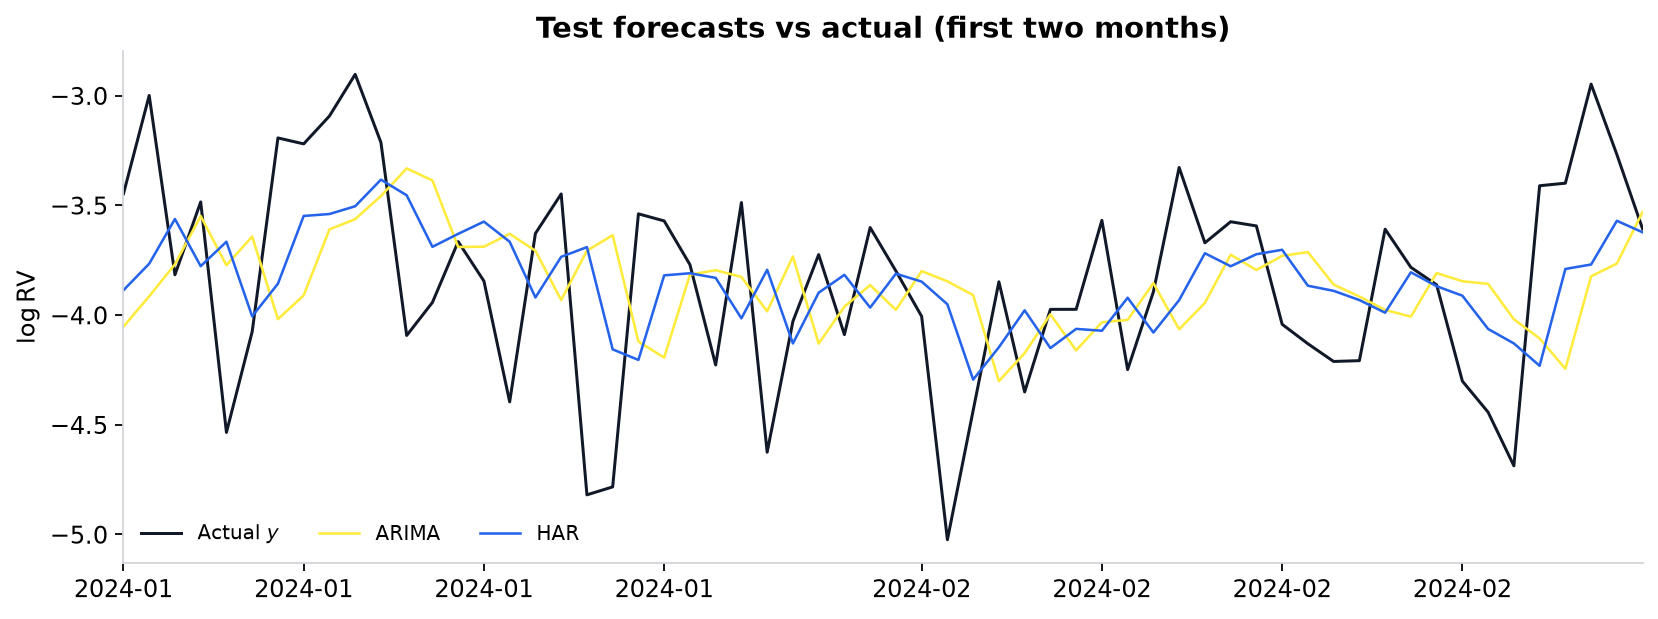
\includegraphics[width=\textwidth]{figures/baseline_test_paths_2mo.png}
\caption{Test path, first two months (2024-01 through 2024-02).}
\end{figure}
\begin{figure}[H]
\centering
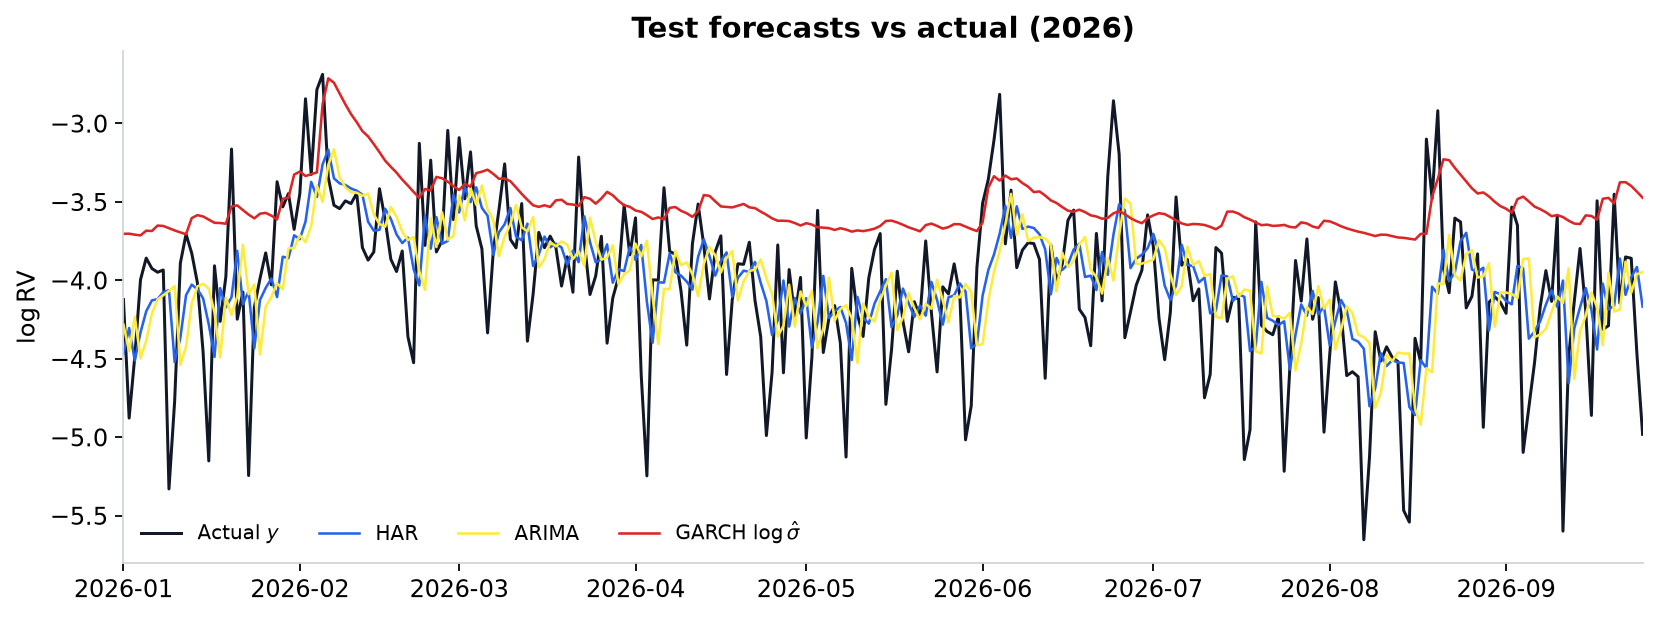
\includegraphics[width=\textwidth]{figures/baseline_test_paths.png}
\caption{Test path in calendar 2026.}
\end{figure}
\begin{explain}
Among the classical models, HAR has the lowest test error. ARIMA improves on Naive. GARCH matches Naive on QLIKE and is higher on log-error.
\end{explain}

\section{Artifacts}
\begin{itemize}
  \item \texttt{models/baseline\_stats.json}
  \item \texttt{models/baseline\_forecasts.parquet}
  \item \texttt{models/run\_baselines.py}
\end{itemize}

\section{Next}
LSTM under the same Protocol~B and the same test metrics.

\end{document}
